\documentclass[12pt,a4paper]{report}
\usepackage{graphicx}
\usepackage[
sorting=none
]{biblatex}
\addbibresource{references.bib}

\begin{document}
  \par
    One of the main goals of the curator of the Rijksmuseum is to make artwork meaningful for the public. This usually takes place in the form of lectures, publications or carefully crafted exhibitions. A visit to the museum should lead to inspiring conversations and discussions about how we can see the world in different and unexpected ways. We believe that leveraging artificial intelligence (AI) to interface with the Rijksmuseum’s Open Access online collection, will contribute significantly to how the people experience the museum’s collection. This also would allow us to visualise the structure underlying artistic creation itself.

  \par
    As a first step in the direction of exploring and classifying the dataset of photographic reproductions of the artworks exhibited in the Rijksmuseum, the Machine Learning team of the Netherlands eScience Center, is currently working on the Museum-Centered Visual Recognition Challenge \cite{Mensink2014}. Here, we aim to classify the images using a convolutional neural network based on the artist, the type of art, the material used and the creation year. This would improve the tools of a museum curator while also improving content-based exploration by online visitors of the museum collection. If significant progress is made, the model can be used to classify unidentified paintings.

  \par
    Once the groundwork of classifying images is laid, it paves way to a multitude of opportunities in terms of applications. One could think of ways of coupling the model to social media which would match the photos that people post with artwork from the museum. For instance, a photo of an afternoon tea party can be complemented with Ayaoka Yûshin’s Theeservies, as shown in Fig. \ref{ai}.

    \begin{figure}[h]
      \centering
      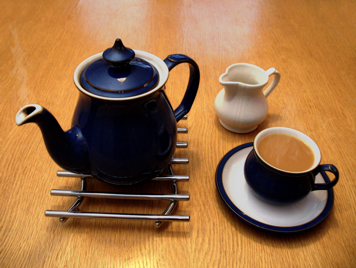
\includegraphics{tea.png}
      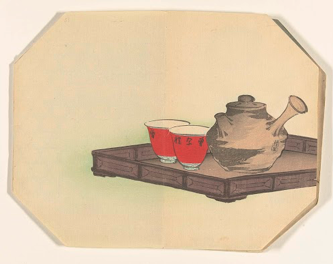
\includegraphics{tea2.png}
      \caption{AI matches images on social media with artwork from the museum's collection to make the artwork more personal.}
      \label{ai}
    \end{figure}

  \par
    Yet another way to incorporate the artworks in everyday life is to use voice recognition AI to follow a discussion and share artworks from the collection that resonate with the stories being told. The generated series of artworks can be shared on social media along with the story itself, and the AI can generate a tour of the museum based on the artworks selected. This potentially opens up interest in lesser visited parts of the museum.

  \par
    AI can also help us to understand the underlying creative process. Generative Adversarial Networks (GANs are a type of deep neural network) can be used to generate paintings in the style of any artist. Hence, we can see the same subject as painted by Rembrandt or Van Gogh, which would give us a better understanding of how art evolved.

    \printbibliography

\end{document}
